%Author: Anil Zenginoglu
\documentclass[border=3pt,tikz]{standalone}
\usepackage{tikz}
\usepackage{amsmath} % for \text
\usepackage{mathrsfs} % for \mathscr -> scri
\usetikzlibrary{decorations.pathmorphing} % for the singularity zigzag
\usepackage{pgfplots}

\begin{document}
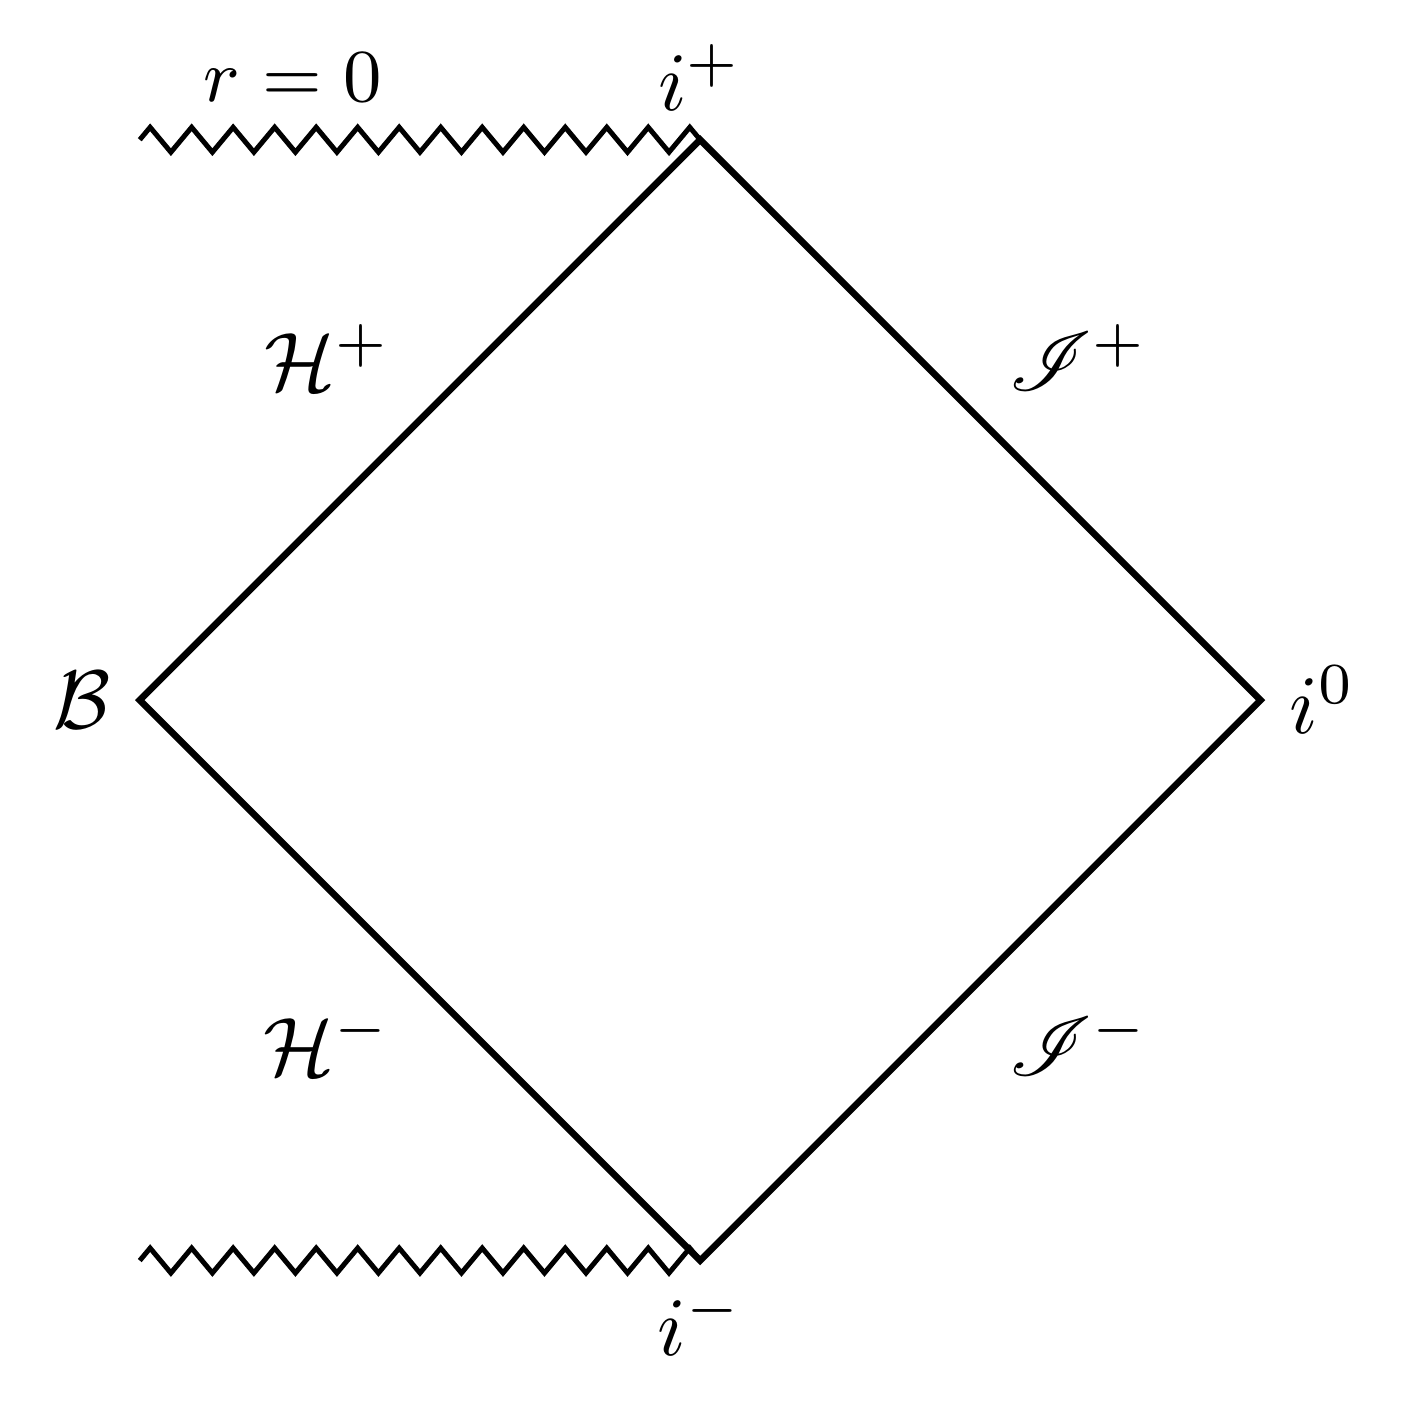
\begin{tikzpicture}[scale=3]
 \begin{axis}[axis lines=none, xmin=-.2,xmax=2.2,ymin=-1.2,ymax=1.2,width=0.6\textwidth,height=0.6\textwidth]

    % BOUNDING DIAGRAM
    \coordinate (O)  at (axis cs:1, 0); % center I: origin (r,t) = (0,0)
    \coordinate (S)  at (axis cs: 1,-1); % south I: t=-infty, i-
    \coordinate (N)  at (axis cs: 1, 1); % north I: t=+infty, i+
    \coordinate (E)  at (axis cs: 2, 0); % east I:  r=-infty, i0
    \coordinate (W)  at (axis cs: 0, 0); % west: bifurcation
    \coordinate (NW) at (axis cs:0,1); 
    \coordinate (SW) at (axis cs:0,-1);
    \draw[line width=0.6,decorate, 
        decoration={zigzag,amplitude=1.5,segment length=5}] 
        (NW) -- node[above left=1] {\small{$r=0$}} (N);
    \draw[line width=0.6,decorate, 
        decoration={zigzag,amplitude=1.5,segment length=5}] 
        (SW) -- (S);

    \draw[thick] (N) -- (E) -- (S) -- (W) -- cycle;
    
    % LABELS
    \newcommand{\scri}{\mathscr{I}}
    \node[right] at (E) {$i^0$};
    \node[above] at (N) {$i^+$};
    \node[below] at (S) {$i^-$};
    \node[above right] at (axis cs:1.5,0.5) {$\scri^+$};
    \node[below right] at (axis cs:1.5,-0.5) {$\scri^-$};
    \node[above left] at (axis cs:0.5,0.5) {$\mathcal{H}^+$};
    \node[below left] at (axis cs:0.5,-0.5) {$\mathcal{H}^-$};
    \node[left] at (W) {$\mathcal{B}$};
    
%     \foreach \file in {
% {data/ss0.csv},
% {data/ss1.csv},
% {data/ss2.csv},
% {data/ss3.csv},
% {data/ss4.csv},
% {data/ss5.csv},
% {data/ss6.csv}
% }
%     	{\addplot[domain={-1,1}] table [x=R, y=T, col sep=comma] {\file};}


\end{axis}
\end{tikzpicture}

\end{document}



%\addplot[domain={-1,1}] table [x=R, y=T, col sep=comma] {arctan_data12.csv};
